%%%%%%%%%%%%%%%%%%%%%%%%%%%%%%%%%%%%%%%%%
% Journal Article
% LaTeX Template
% Version 2.0 (February 7, 2023)
%
% This template originates from:
% https://www.LaTeXTemplates.com
%
% Author:
% Vel (vel@latextemplates.com)
%
% License:
% CC BY-NC-SA 4.0 (https://creativecommons.org/licenses/by-nc-sa/4.0/)
%
% NOTE: The bibliography needs to be compiled using the biber engine.
%
%%%%%%%%%%%%%%%%%%%%%%%%%%%%%%%%%%%%%%%%%

%----------------------------------------------------------------------------------------
%	PACKAGES AND OTHER DOCUMENT CONFIGURATIONS
%----------------------------------------------------------------------------------------

\documentclass[
	a4paper, % Paper size, use either a4paper or letterpaper
	10pt, % Default font size, can also use 11pt or 12pt, although this is not recommended
	unnumberedsections, % Comment to enable section numbering
	twoside, % Two side traditional mode where headers and footers change between odd and even pages, comment this option to make them fixed
]{LTJournalArticle}

\usepackage{amsmath}

\addbibresource{sample.bib} % BibLaTeX bibliography file

\runninghead{Recipy - Búsqueda de Recetas} % A shortened article title to appear in the running head, leave this command empty for no running head

\footertext{\textit{Artículo para Posgrado de Redes Complejas} (2023)} % Text to appear in the footer, leave this command empty for no footer text

\setcounter{page}{1} % The page number of the first page, set this to a higher number if the article is to be part of an issue or larger work

%----------------------------------------------------------------------------------------
%	TITLE SECTION
%----------------------------------------------------------------------------------------

\title{Recipy\\Motor de búsqueda de recetas usando grafos} % Article title, use manual lines breaks (\\) to beautify the layout

% Authors are listed in a comma-separated list with superscript numbers indicating affiliations
% \thanks{} is used for any text that should be placed in a footnote on the first page, such as the corresponding author's email, journal acceptance dates, a copyright/license notice, keywords, etc
\author{%
	Luis Ibarra\textsuperscript{1} y Marcos Valdivié\textsuperscript{1} 
	% Jane Smith\textsuperscript{1}\thanks{Corresponding author: \href{mailto:jane@smith.com}{jane@smith.com}\\ \textbf{Received:} October 20, 2023, \textbf{Published:} December 14, 2023}
}

% Affiliations are output in the \date{} command
\date{\footnotesize\textsuperscript{\textbf{1}}Facultad de Matemática y Computación, Universidad de La Habana}

% Full-width abstract
\renewcommand{\maketitlehookd}{%
	\begin{abstract}
		\noindent Lorem ipsum dolor sit amet, consectetur adipiscing elit. Praesent porttitor arcu luctus, imperdiet urna iaculis, mattis eros. Pellentesque iaculis odio vel nisl ullamcorper, nec faucibus ipsum molestie. Sed dictum nisl non aliquet porttitor. Etiam vulputate arcu dignissim, finibus sem et, viverra nisl. Aenean luctus congue massa, ut laoreet metus ornare in. Nunc fermentum nisi imperdiet lectus tincidunt vestibulum at ac elit. Nulla mattis nisl eu malesuada suscipit. Aliquam arcu turpis, ultrices sed luctus ac, vehicula id metus. Morbi eu feugiat velit, et tempus augue. Proin ac mattis tortor. Donec tincidunt, ante rhoncus luctus semper, arcu lorem lobortis justo, nec convallis ante quam quis lectus. Aenean tincidunt sodales massa, et hendrerit tellus mattis ac. Sed non pretium nibh. Donec cursus maximus luctus. Vivamus lobortis eros et massa porta porttitor.
	\end{abstract}
}

%----------------------------------------------------------------------------------------

\begin{document}

\maketitle % Output the title section

%----------------------------------------------------------------------------------------
%	ARTICLE CONTENTS
%----------------------------------------------------------------------------------------

\section{Introduction}

Lorem ipsum dolor sit amet, consectetur adipiscing elit. Praesent porttitor arcu luctus, imperdiet urna iaculis, mattis eros. Pellentesque iaculis odio vel nisl ullamcorper, nec faucibus ipsum molestie. Sed dictum nisl non aliquet porttitor. Etiam vulputate arcu dignissim, finibus sem et, viverra nisl. Aenean luctus congue massa, ut laoreet metus ornare in. Nunc fermentum nisi imperdiet lectus tincidunt vestibulum at ac elit. Nulla mattis nisl eu malesuada suscipit.

Aliquam arcu turpis, ultrices sed luctus ac, vehicula id metus. Morbi eu feugiat velit, et tempus augue. Proin ac mattis tortor. Donec tincidunt, ante rhoncus luctus semper, arcu lorem lobortis justo, nec convallis ante quam quis lectus. Aenean tincidunt sodales massa, et hendrerit tellus mattis ac. Sed non pretium nibh. Donec cursus maximus luctus. Vivamus lobortis eros et massa porta porttitor. Donec laoreet nisl vel risus lacinia elementum non nec lacus. Nullam luctus, nulla volutpat ultricies ultrices, quam massa placerat augue, ut fringilla urna lectus nec nibh. Vestibulum efficitur condimentum orci a semper. Pellentesque ut metus pretium lacus maximus semper.

Fusce varius orci ac magna dapibus porttitor. In tempor leo a neque bibendum sollicitudin. Nulla pretium fermentum nisi, eget sodales magna facilisis eu. Praesent aliquet nulla ut bibendum lacinia. Donec vel mauris vulputate, commodo ligula ut, egestas orci. Suspendisse commodo odio sed hendrerit lobortis. Donec finibus eros erat, vel ornare enim mattis et. Donec finibus dolor quis dolor tempus consequat. Mauris fringilla dui id libero egestas, ut mattis neque ornare. Ut condimentum urna pharetra ipsum consequat, eu interdum elit cursus. Vivamus scelerisque tortor et nunc ultricies, id tincidunt libero pharetra. Aliquam eu imperdiet leo. Morbi a massa volutpat velit condimentum convallis et facilisis dolor.

\begin{equation}
	\cos^3 \theta =\frac{1}{4}\cos\theta+\frac{3}{4}\cos 3\theta
	\label{eq:example}
\end{equation}

Automatically referencing an equation number using its label: Equation \ref{eq:example}.

In hac habitasse platea dictumst. Curabitur mattis elit sit amet justo luctus vestibulum. In hac habitasse platea dictumst. Pellentesque lobortis justo enim, a condimentum massa tempor eu. Ut quis nulla a quam pretium eleifend nec eu nisl. Nam cursus porttitor eros, sed luctus ligula convallis quis. Nam convallis, ligula in auctor euismod, ligula mauris fringilla tellus, et egestas mauris odio eget diam. Praesent sodales in ipsum eu dictum. Aenean vel enim ipsum. Fusce ut felis at eros sagittis bibendum mollis lobortis libero.

Maecenas consectetur metus at tellus finibus condimentum. Proin arcu lectus, ultrices non tincidunt et, tincidunt ut quam. Integer luctus posuere est, non maximus ante dignissim quis. Nunc a cursus erat. Curabitur suscipit nibh in tincidunt sagittis. Nam malesuada vestibulum quam id gravida. Proin ut dapibus velit. Vestibulum eget quam quis ipsum semper convallis. Duis consectetur nibh ac diam dignissim, id condimentum enim dictum. Nam aliquet ligula eu magna pellentesque, nec sagittis leo lobortis. Aenean tincidunt dignissim egestas.

%------------------------------------------------

\section{Desarrollo}

\subsection{Grafos}

Para la conformación de la base de datos para el motor de búsqueda se contruyen diferentes grafos que
contienen información relacionada a la interacción entre los componentes que de una manera u otra conforman
las recetas.

\subsubsection{Grafo Bipartito Receta-Ingrediente}

Se define como un grafo no dirigido en el cual sus nodos representan
recetas o ingredientes y sus aristas representan la participación de un ingrediente en la confección de la receta.
Dado que el grafo en bipartito, no se permiten las aristas entre ingredientes ni entre recetas.

En este grafo, el grado (\textit{degree}) del nodo representa la cantidad de recetas que necesitan
el ingrediente dado, y de manera recíproca también representa la cantidad de ingredientes utilizados para 
confeccionar la receta dada.

\subsubsection{Grafo Bipartito Ingrediente-Acción}

TODO

\subsubsection{Grafo Receta-Receta}

Se define como un grafo no dirigido en el cual sus nodos representan recetas y sus aristas
están ponderadas con una métrica de similitud entre recetas. Para este tipo de grafo se confeccionaron dos 
versiones basadas en diferentes métricas:

\begin{enumerate}
	\item Similitud de Jaccard entre los conjuntos de ingredientes utilizados por ambas recetas.
	\item Similitud vectorial entre representación semántica de recetas.
\end{enumerate}

\textbf{Similitud de Jaccard}

Para la confección de este grafo las aristas son ponderadas mediante la similitud de Jaccard (Ecuación \ref{eq:jaccard_sim}).

\begin{equation}
	J(A, B) = \frac{|A \cap B|}{|A \cup B|}
	\label{eq:jaccard_sim}
\end{equation}

\begin{enumerate}
	\item Se representaron las recetas como el conjunto de ingredientes que se necesitan para ser preparadas.
	\item Se calcula la similitud de Jaccard para cada par de nodos obteniendo el peso de la arista correspondiente.
\end{enumerate}

\textbf{Similitud vectorial entre representación semántica de recetas}

Para la confección de este grafo se realizaron un conjunto de pasos para la vectorización semántica de las recetas.

\begin{enumerate}
	\item Se representaron las recetas como una lista de las instrucciones de su preparación.
	\item Cada instrucción fue codificada por el modelo \textit{Universal Sentence Encoder} \autocite{Smith:2023qr}
	el cual devuelve un vector de dimensión 512 por cada oración procesada, obteniendo una representación final
	para la receta con dimensión $(CantInstrucciones, 512)$. 
	\item Se procedió a disminuir la dimensión hasta un vector de dimensión 256. Esto se logra mediante un 
	entrenamiento no supervisado con modelo encoder-decoder (Figura \ref{fig:encoder_decoder_small}).
	\item Para el peso de las aristas se utiliza la similitud de exponencial inversa de la distancia entre vectores 
	(Ecuación \ref{eq:inverse_exp_sim})
\end{enumerate}

\begin{equation}
	invExpSim(x, y) = e^{-||x-y||}
	\label{eq:inverse_exp_sim}
\end{equation}

\begin{figure}
	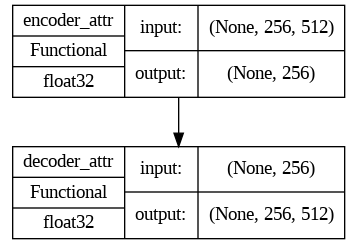
\includegraphics[width=\linewidth]{full_model.png}
	\caption{Arquitectura encoder-decoder para el vectorización de recetas.}
	\label{fig:encoder_decoder_small}
\end{figure}

\subsubsection{Grafo Ingrediente-Ingrediente}

Se define como un grafo no dirigido en el cual sus nodos representan ingredientes y sus aristas
están ponderadas con una métrica de similitud entre ingredientes. 
Para este tipo de grafo se confeccionaron tres versiones basadas en diferentes métricas:

\begin{enumerate}
	\item Similitud de Jaccard entre los conjuntos de recetas utilizados por ambos ingredientes.
	\item Similitud vectorial entre representación sintáctica de ingredientes mediante vectorización 
	por frecuencia de términos.
	\item Similitud por \textit{Pointwise mutual information} (PMI) definida en \textcite{teng2012recipe}.
\end{enumerate}

\textbf{Similitud de Jaccard}

La confección de este grafo se realiza de manera similar a su contraparte de recetas.

\begin{enumerate}
	\item Los ingredientes se representan por el conjunto de recetas en los que se usan.
	\item Se calcula la similitud de Jaccard (Ecuación \ref{eq:jaccard_sim}) entre ingredientes para ponderar las aristas
	entre estos.
\end{enumerate}

Este grafo provee información acerca de cómo están asociados los ingredientes con las recetas. Una valor de similitud
cercano a 1 indica que los ingredientes pertenecientes a la arista se comparten en la mayoría de las recetas en que son
utilizados. En caso de estar cercano a 0, indica que no coinciden en casi ninguna receta dichos ingredientes.

\textbf{Similitud vectorial entre representación sintáctica de ingredientes}

En la confección de este grafo se realiza una transformación del nombre de los ingredientes a vectores mediante
un conteo de las palabras presentes en su nombre.

\begin{enumerate}
	\item Cada ingrediente se representa por su nombre.
	\item Los nombres son vectorizados a una tabla de términos de frecuencia normalizada.
	\item Las aristas entre los ingredientes son ponderadas por la similitud de coseno entre las 
	representaciones vectoriales de cada par de ingredientes.
\end{enumerate}

Una razón por la cual construir este grafo es para dar información acerca de las diferentes variantes de ingredientes.
Estas distintas variantes, por lo general poseen nombres compuestos con la clase principal en su nombre, por ejemplo:

\begin{itemize}
	\item Queso
	\item Queso Parmesano
	\item Queso Ravioli
	\item Queso Gouda
\end{itemize}

\textbf{Similitud por PMI}

En la confección de este grafo se calcula el PMI \autocite{teng2012recipe} (Ecuación \ref{eq:pmi}) entre cada par de ingredientes:

\begin{equation}
	PMI(a, b) = \log \frac{p(a,b)}{p(a)p(b)},
	\label{eq:pmi}
\end{equation}

donde

\begin{equation*}
	p(a) = \frac{\text{\# de recetas que contienen \textit{a}}}{\text{\# de recetas}},
\end{equation*}
\begin{equation*}
	p(a,b) = \frac{\text{\# de recetas que contienen \textit{a} y \textit{b}}}{\text{\# de recetas}}.
\end{equation*}

\begin{enumerate}
	\item Cada ingrediente es representado por el conjunto de recetas en el cual es utilizado.
	\item Se calcula el PMI entre cada par de ingredientes y se pondera la arista con este valor.
\end{enumerate}

En este grafo, los pesos pueden llegar a ser negativos o positivos. En este caso nos interesa los pesos positivos,
ya que estos pesos indican que la probabilidad de que coincidan dos ingredientes al mismo tiempo es mayor que la
probabilidad que coincidan de forma independiente, por lo tanto su ocurrencia está condicionada a ser más probable
dado que tengo un ingrediente.

$$
PMI(a,b) = \log \frac{p(a,b)}{p(a)p(b)} > 0
$$
$$
\frac{p(a,b)}{p(a)p(b)} > 1
$$
$$
p(a,b) > p(a)p(b)
$$
$$
p(a|b)p(b) > p(a)p(b) \quad p(b|a)p(a) > p(a)p(b)
$$
$$
p(a|b) > p(a) \quad p(b|a) > p(b)
$$
	
\subsection{Ranking de Nodos}

Dada la cantidad de nodos presentes en los grafos, en algunas situaciones existe la necesidad de reducir esta
cantidad. Para esto se toman diferentes estrategias en dependencia del tipo de grafo con el que se trabaje:

\begin{enumerate}
	\item Ranking de recetas por valoraciones de usuarios.
	\item Ranking de ingredientes por ocurrencias acumuladas.
\end{enumerate}

\textbf{Ranking de recetas por valoraciones de usuarios}

Dado un conjunto de valoraciones a recetas dadas por usuarios se procede a definir 
una medida de importancia con estas. Para esto se realizan los siguintes pasos:

\begin{enumerate}
	\item Se extraen para cada receta la cantidad de valoraciones y la media de estas.
	\item Dichos valores son normalizados entre 0 y 1 al dividirlos por la cantidad máxima de ambas métricas por receta.
	\item Se calcula la métrica F1 entre ambos valores para obtener la importancia final de la receta (Ecuación \ref{eq:f1_recipe_rank}).
\end{enumerate}

\begin{equation}
	ImpReceta(r, Val) = F1(A(r, Val), M(r, Val)),
	\label{eq:f1_recipe_rank}
\end{equation}

donde

\begin{equation*}
	F1(a, b) = 2 \frac{a · b}{a + b},
\end{equation*}

\begin{equation*}
	A(r, Val) = \frac{|[r \sqsubseteq Val]|}{\max \{\,|[p \sqsubseteq Val]| \, \vert \, p \in R \, \}},
\end{equation*}

\begin{equation*}
	M(r, Val) = \frac{mean([r \sqsubseteq Val])}{\max \{\,mean([p \sqsubseteq Val]) \, \vert \, p \in R\,\}},
\end{equation*}

$Val$ es la lista de valoraciones dadas por los usuarios, la expresión $[r \sqsubseteq Val]$ denota la lista de valores de 
las valoraciones dadas a la receta $r$ y $R$ es el conjunto de recetas.

Esta métrica previene que recetas con pocas y muy altas valoraciones tengan más importancia que recetas con muchas
valoraciones pero más bajas. De manera que las recetas más importantes tengan que tener al mismo tiempo una gran 
cantidad de valoraciones y que estas sean buenas. 

\textbf{Ranking de ingredientes por ocurrencias acumuladas}

Dado un conjunto de ingredientes se toman los que participan en la mayor cantidad de enlaces entre recetas.
Para realizar el ranking se realizan los siguientes pasos:

\begin{enumerate}
	\item Ordenar por grado de mayor a menor los nodos ingredientes del grafo bipartito de ingredientes-recetas.
	\item Seleccionar los ingredientes hasta que la suma total de los grados de los nodos seleccionados represente
	un porciento fijo de la suma total de todos los grados del grafo.
\end{enumerate}

\subsection{Ranking de Resultados a Consultas}

Para la extracción de ingredientes y recetas dadas una consulta se emplean dos mecanismos para hacer el cálculo
de la relevancia.

\begin{itemize}
	\item Distancia de Levenshtein: Se calcula la distancia de Levenshtein entre la consulta y el nombre de la 
	entidad a extraer.
	\item Similitud Vectorial: Se calcula la similitud de coseno entre la vectorización de la consulta y los
	vectores de la entidad. Las entidades son vectorizadas mediante una tabla TF-IDF. 
\end{itemize}

\section{Experimentación y Resultados}

Para la confección del motor de búsqueda de recetas se conformó un paquete de Python, \textbf{recipy}, el cual
contiene las funciones necesarias para la creación de grafos y consulta de grafos. Para la visualización de los
resultados se creó una aplicación usando \textbf{streamlit} la cual permite al usuario interactuar con la API.

\subsection{Datos}

Se trabajaron con tres conjuntos de datos cada uno provisto con diferentes elementos (Tabla \ref{tab:data_features}):

\begin{itemize}
	\item Cocina al Minuto
	\item Food.com \autocite{majumder2019generating}
	\item RecipeNLG \autocite{bien-etal-2020-recipenlg}
\end{itemize}

\begin{table*} % Single column table
	\caption{Atributos de los conjuntos de datos.}
	\centering
	\begin{tabular}{l l l l}
		\toprule
		Atributo 				 & Cocina al Minuto & Food.com & RecipeNLG  \\
		\midrule
		Cantidad de Recetas 	 & 555				& 230,186	& 1,312,871	\\
		Cantidad de Ingredientes & 214	 			& 14,927	& 170,204	\\
		Cantidad de Pasos 		 & -	 			& 2,248,564	& 9,709,075	\\
		Cantidad de Comentarios  & -	 			& 1,132,367	&	-		\\
		\bottomrule
	\end{tabular}
	\label{tab:data_features}
\end{table*}

%------------------------------------------------

\section{Results}

\begin{table} % Single column table
	\caption{Example single column table.}
	\centering
	\begin{tabular}{l l r}
		\toprule
		\multicolumn{2}{c}{Location} \\
		\cmidrule(r){1-2}
		East Distance & West Distance & Count \\
		\midrule
		100km & 200km & 422 \\
		350km & 1000km & 1833 \\
		600km & 1200km & 890 \\
		\bottomrule
	\end{tabular}
	\label{tab:distcounts}
\end{table}

Referencing a table using its label: Table \ref{tab:distcounts}.

\begin{table*} % Full width table (notice the starred environment)
	\caption{Example two column table with fixed-width columns.}
	\centering % Horizontally center the table
	\begin{tabular}{L{0.2\linewidth} L{0.2\linewidth} R{0.15\linewidth}} % Manually specify column alignments with L{}, R{} or C{} and widths as a fixed amount, usually as a proportion of \linewidth
		\toprule
		\multicolumn{2}{c}{Location} \\
		\cmidrule(r){1-2}
		East Distance & West Distance & Count \\
		\midrule
		100km & 200km & 422 \\
		350km & 1000km & 1833 \\
		600km & 1200km & 890 \\
		\bottomrule
	\end{tabular}
\end{table*}

Aenean feugiat pellentesque venenatis. Sed faucibus tristique tortor vel ultrices. Donec consequat tellus sapien. Nam bibendum urna mauris, eget sagittis justo gravida vel. Mauris nisi lacus, malesuada sit amet neque ut, venenatis tempor orci. Curabitur feugiat sagittis molestie. Duis euismod arcu vitae quam scelerisque facilisis. Praesent volutpat eleifend tortor, in malesuada dui egestas id. Donec finibus ac risus sed pellentesque. Donec malesuada non magna nec feugiat. Mauris eget nibh nec orci congue porttitor vitae eu erat. Sed commodo ipsum ipsum, in elementum neque gravida euismod. Cras mi lacus, pulvinar ut sapien ut, rutrum sagittis dui. Donec non est a metus varius finibus. Pellentesque rutrum pellentesque ligula, vitae accumsan nulla hendrerit ut.

\begin{figure} % Single column figure
	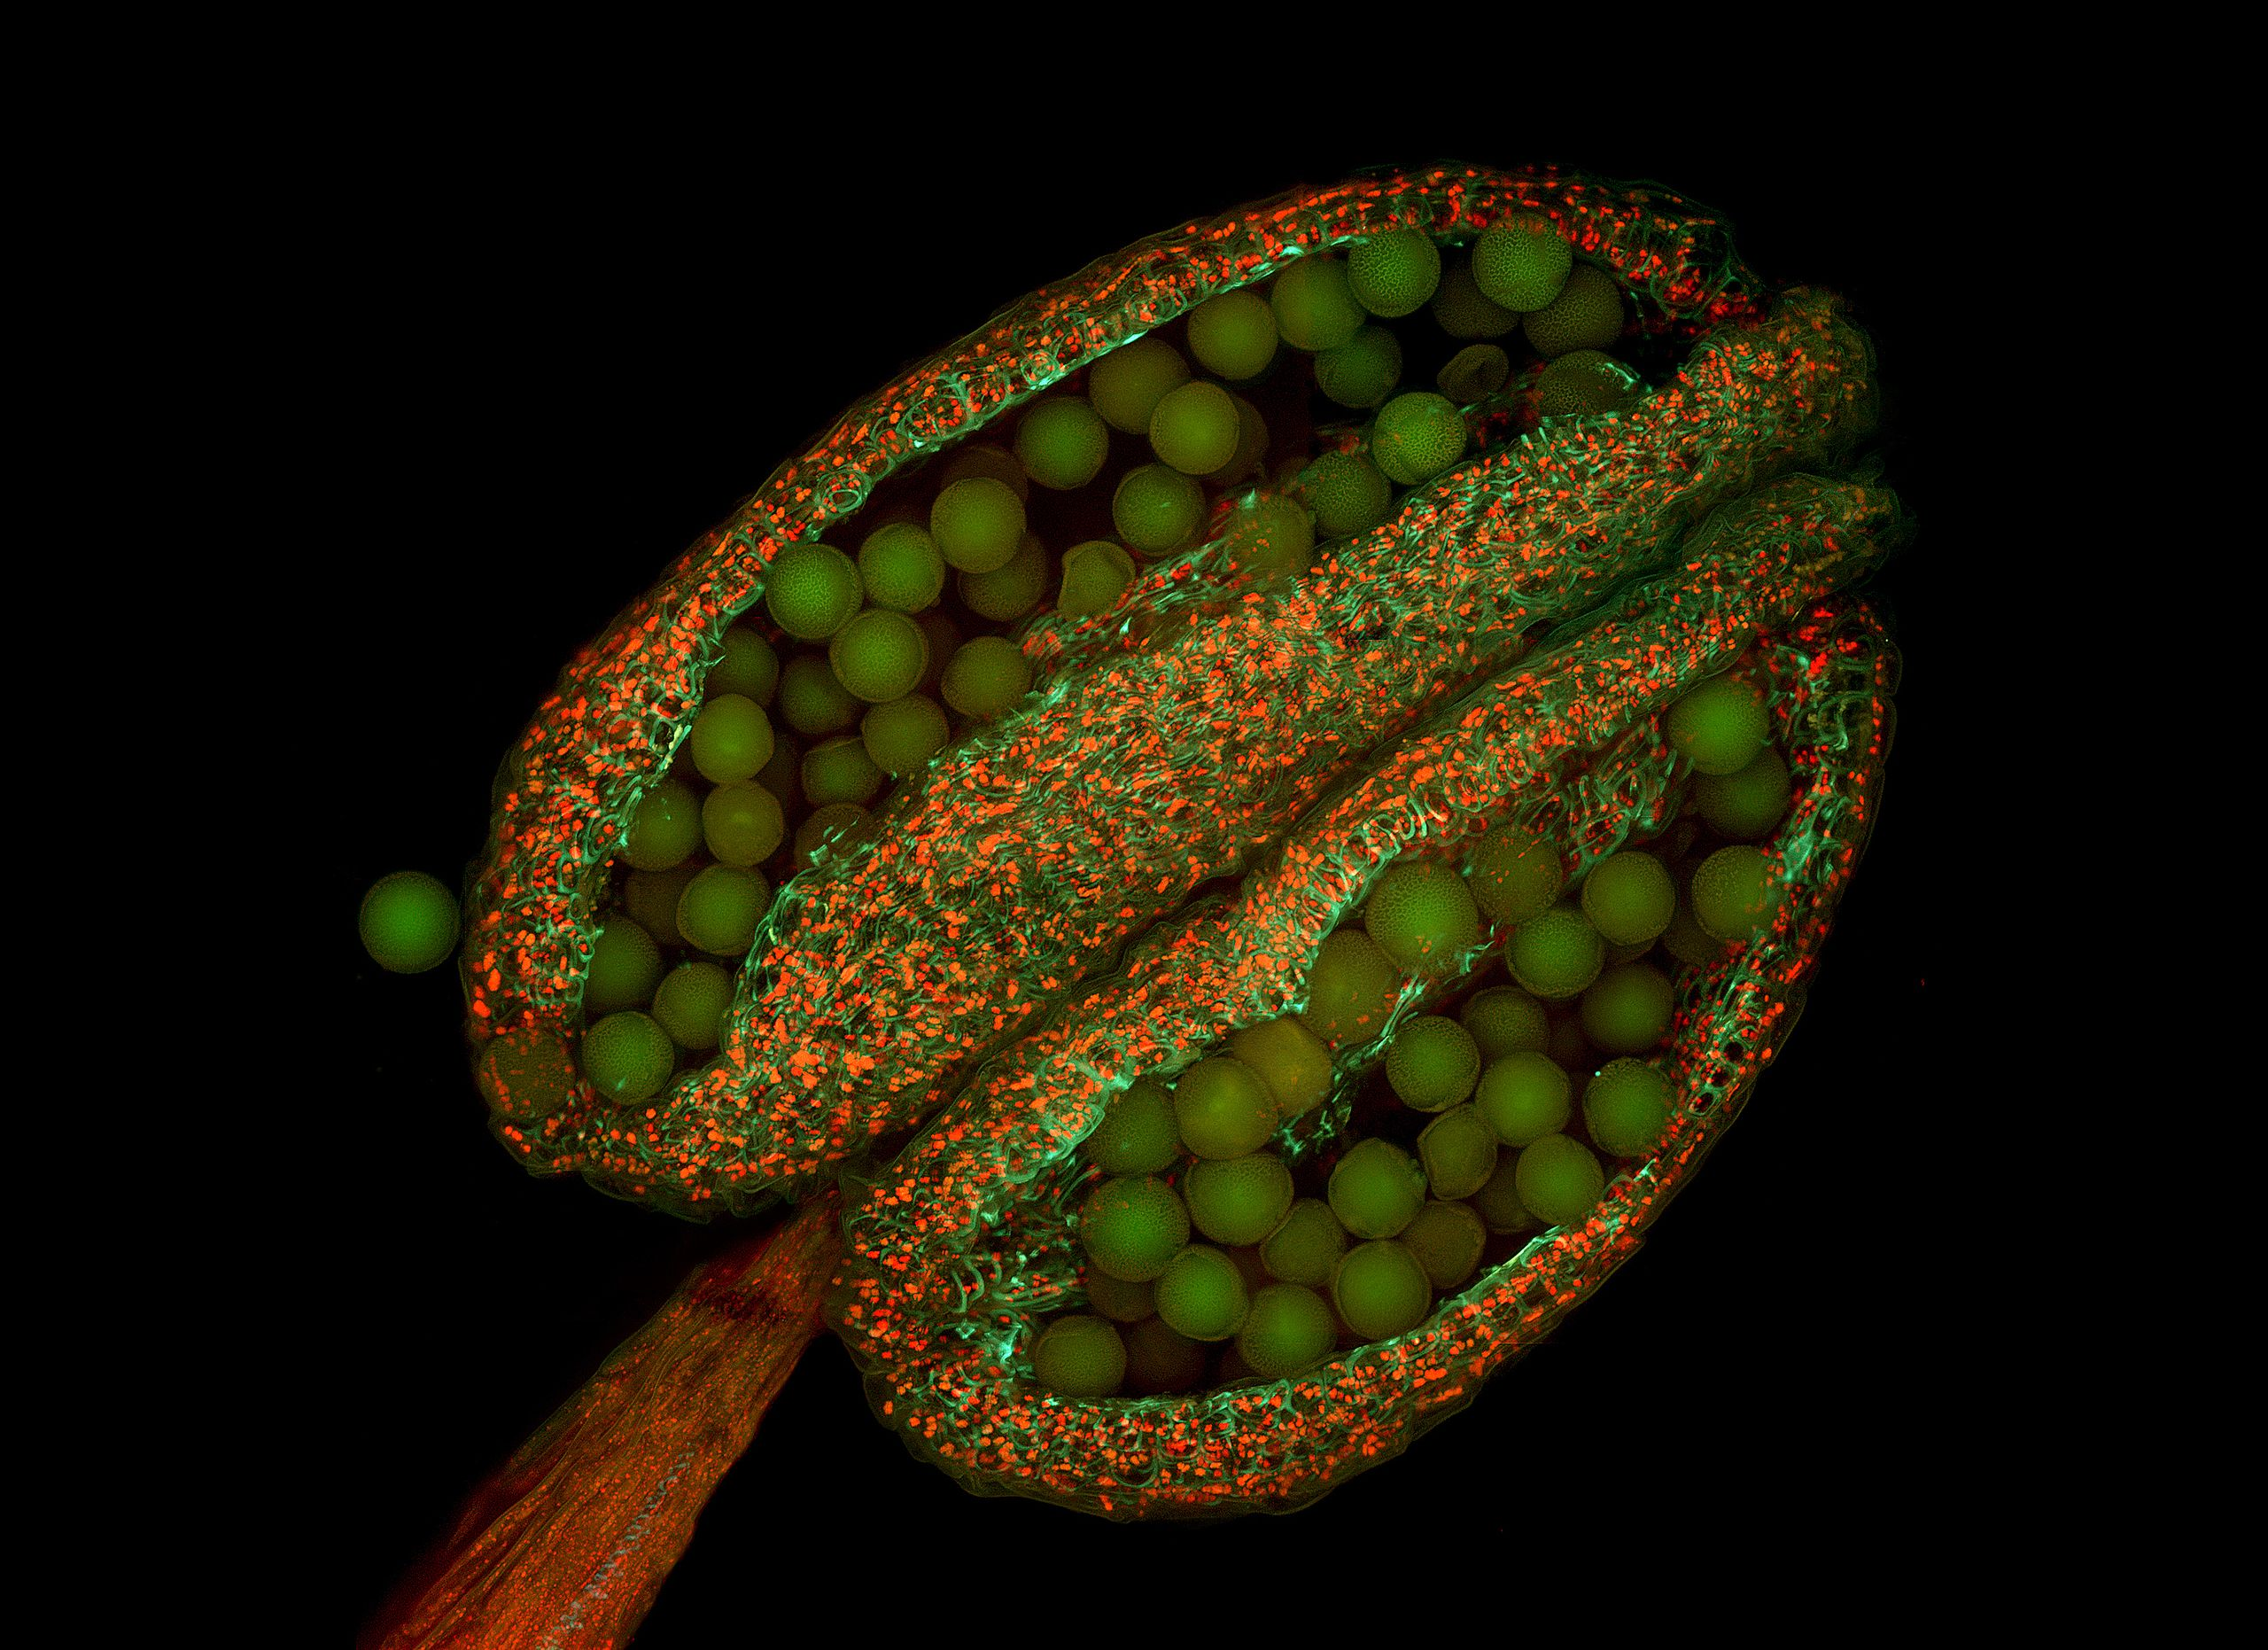
\includegraphics[width=\linewidth]{Tolmukapea.jpg}
	\caption{Anther of thale cress (Arabidopsis thaliana), fluorescence micrograph. Source: Heiti Paves, \href{https://commons.wikimedia.org/wiki/File:Tolmukapea.jpg}{https://commons.wiki-\\media.org/wiki/File:Tolmukapea.jpg}.}
	\label{fig:tcanther}
\end{figure}

Referencing a figure using its label: Figure \ref{fig:tcanther}.

Aenean porttitor eros non pharetra congue. Proin in odio in dolor luctus auctor ac et mi. Etiam euismod mi sed lectus fringilla pretium. Phasellus tristique maximus lectus et sodales. Mauris feugiat ligula quis semper luctus. Nam sit amet felis sed leo fermentum aliquet. Mauris arcu dui, posuere id sem eget, cursus pulvinar mi. Donec nec lacus non lectus fermentum scelerisque et at nibh. Sed tristique, metus ac vestibulum porta, tortor lectus placerat lorem, et convallis tellus dolor eget ante. Pellentesque dui ligula, hendrerit a purus et, volutpat tempor lectus. Mauris nec purus nec mauris rhoncus pellentesque. Quisque quis diam sed est lacinia congue. Donec magna est, hendrerit sed metus vel, accumsan rutrum nibh.

\begin{figure*} % Two column figure (notice the starred environment)
	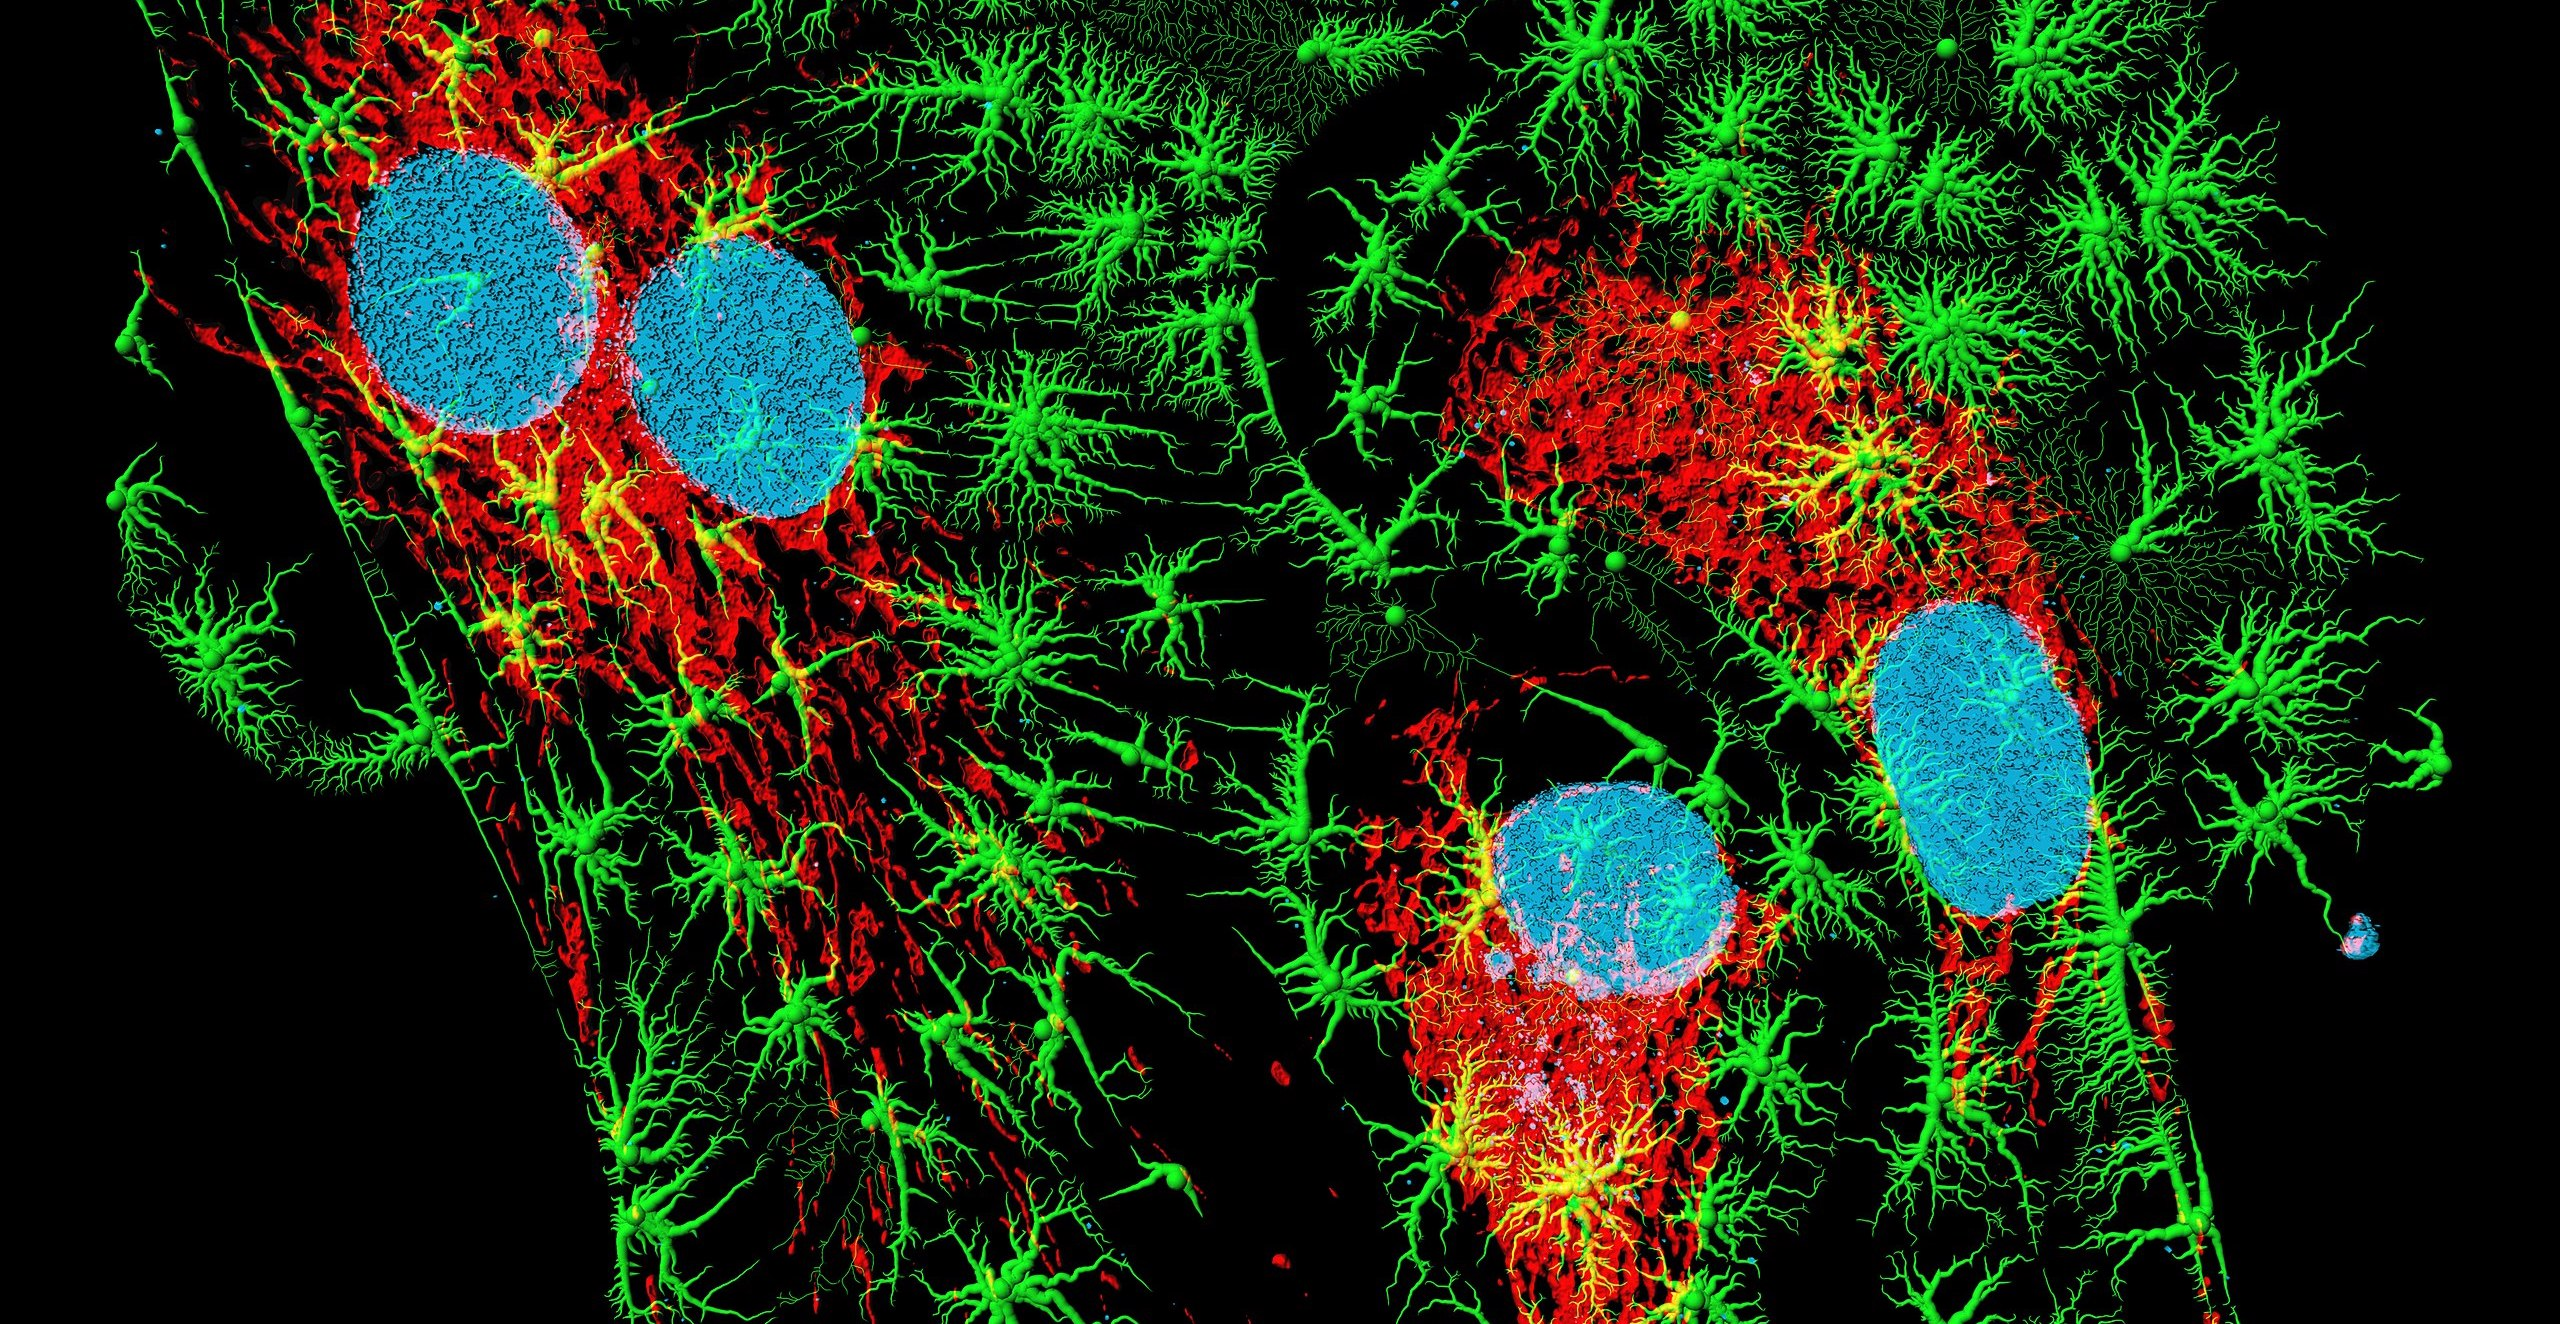
\includegraphics[width=\linewidth]{Fibroblastid.jpg}
	\caption{Bovine pulmonary artery endothelial cells in culture. Blue: nuclei; red: mitochondria; green: microfilaments. Computer generated image from a 3D model based on a confocal laser scanning microscopy using fluorescent marker dyes. Source: Heiti Paves, \href{https://commons.wikimedia.org/wiki/File:Fibroblastid.jpg}{https://commons.wikimedia.org/wiki/File:Fibroblastid.jpg}.}
	\label{fig:bpartery}
\end{figure*}

Orci varius natoque penatibus et magnis dis parturient montes, nascetur ridiculus mus. Etiam cursus lectus purus, tempus iaculis quam dictum tristique. Nam interdum sapien nec tempor mattis. Quisque id sapien nisi. Mauris vehicula ornare eros vel efficitur. Nulla consectetur, turpis quis fringilla tincidunt, mi neque iaculis lectus, vel commodo elit odio non ex. Duis facilisis, purus ac viverra iaculis, turpis lectus ultrices ante, ac vestibulum ligula magna in libero. Etiam tristique maximus lacinia. Vestibulum hendrerit, lacus malesuada laoreet blandit, sapien velit sollicitudin nunc, eu porttitor urna ligula at lorem. Aliquam faucibus eros in fermentum venenatis. Fusce consectetur congue pellentesque. Suspendisse at nisi sit amet est porttitor cursus. Cras placerat faucibus nunc, a laoreet justo dignissim sit amet.

\subsection{International Support}

\noindent àáâäãåèéêëìíîïòóôöõøùúûüÿýñçčšž

\noindent ÀÁÂÄÃÅÈÉÊËÌÍÎÏÒÓÔÖÕØÙÚÛÜŸÝÑ

\noindent ßÇŒÆČŠŽ

\subsection{Links}

This is a clickable URL link: \href{https://www.latextemplates.com}{LaTeX Templates}. This is a clickable email link: \href{mailto:vel@latextemplates.com}{vel@latextemplates.com}. This is a clickable monospaced URL link: \url{https://www.LaTeXTemplates.com}.

%------------------------------------------------

\section{Discussion}

This statement requires citation \autocite{Smith:2023qr}. This statement requires multiple citations \autocite{Smith:2023qr, Smith:2024jd}. This statement contains an in-text citation, for directly referring to a citation like so: \textcite{Smith:2024jd}.

\subsection{Subsection One}

Suspendisse potenti. Vivamus suscipit dapibus metus. Proin auctor iaculis ex, id fermentum lectus dapibus tristique. Nullam maximus eros eget leo pretium dapibus. Nunc in auctor erat, id interdum risus. Suspendisse aliquet vehicula accumsan. In vestibulum efficitur dictum. Sed ultrices, libero nec fringilla feugiat, elit massa auctor ligula, vehicula tempor ligula felis in lectus. Suspendisse sem dui, pharetra ut sodales eu, suscipit sit amet felis. Donec pretium viverra ante, ac pulvinar eros. Suspendisse gravida consectetur urna. Pellentesque vitae leo porta, imperdiet eros eget, posuere sem. Praesent eget leo efficitur odio bibendum condimentum sit amet vel ex. Nunc maximus quam orci, quis pulvinar nibh eleifend ac. Quisque consequat lacus magna, eu posuere tellus iaculis ac. Sed vitae tortor tincidunt ante sagittis iaculis.

\subsection{Subsection Two}

Nullam mollis tellus lorem, sed congue ipsum euismod a. Donec pulvinar neque sed ligula ornare sodales. Nulla sagittis vel lectus nec laoreet. Nulla volutpat malesuada turpis at ultricies. Ut luctus velit odio, sagittis volutpat erat aliquet vel. Donec ac neque eget neque volutpat mollis. Vestibulum viverra ligula et sapien bibendum, vel vulputate ex euismod. Curabitur nec velit velit. Aliquam vulputate lorem elit, id tempus nisl finibus sit amet. Curabitur ex turpis, consequat at lectus id, imperdiet molestie augue. Curabitur eu eros molestie purus commodo hendrerit. Quisque auctor ipsum nec mauris malesuada, non fringilla nibh viverra. Quisque gravida, metus quis semper pulvinar, dolor nisl suscipit leo, vestibulum volutpat ante justo ultrices diam. Sed id facilisis turpis, et aliquet eros.

\subsubsection{Subsubsection Example}

Duis venenatis eget lectus a aliquet. Integer vulputate ante suscipit felis feugiat rutrum. Aliquam eget dolor eu augue elementum ornare. Nulla fringilla interdum volutpat. Sed tincidunt, neque quis imperdiet hendrerit, turpis sapien ornare justo, ac blandit felis sem quis diam. Proin luctus urna sit amet felis tincidunt, sed congue nunc pellentesque. Ut faucibus a magna faucibus finibus. Etiam id mi euismod, auctor nisi eget, pretium metus. Proin tincidunt interdum mi non interdum. Donec semper luctus dolor at elementum. Aenean eu congue tortor, sed hendrerit magna. Quisque a dolor ante. Mauris semper id urna id gravida. Vestibulum mi tortor, finibus eu felis in, vehicula aliquam mi.

Aliquam arcu turpis, ultrices sed luctus ac, vehicula id metus. Morbi eu feugiat velit, et tempus augue. Proin ac mattis tortor. Donec tincidunt, ante rhoncus luctus semper, arcu lorem lobortis justo, nec convallis ante quam quis lectus. Aenean tincidunt sodales massa, et hendrerit tellus mattis ac. Sed non pretium nibh. 

Donec cursus maximus luctus. Vivamus lobortis eros et massa porta porttitor. Nam vitae suscipit mi. Pellentesque ex tellus, iaculis vel libero at, cursus pretium sapien. Curabitur accumsan velit sit amet nulla lobortis, ut pretium ex aliquam. Proin eget volutpat orci. Morbi eu aliquet turpis. Vivamus molestie urna quis tempor tristique. Proin hendrerit sem nec tempor sollicitudin.

%----------------------------------------------------------------------------------------
%	 REFERENCES
%----------------------------------------------------------------------------------------

\printbibliography % Output the bibliography

%----------------------------------------------------------------------------------------

\section{Anexos}

\begin{figure*}
	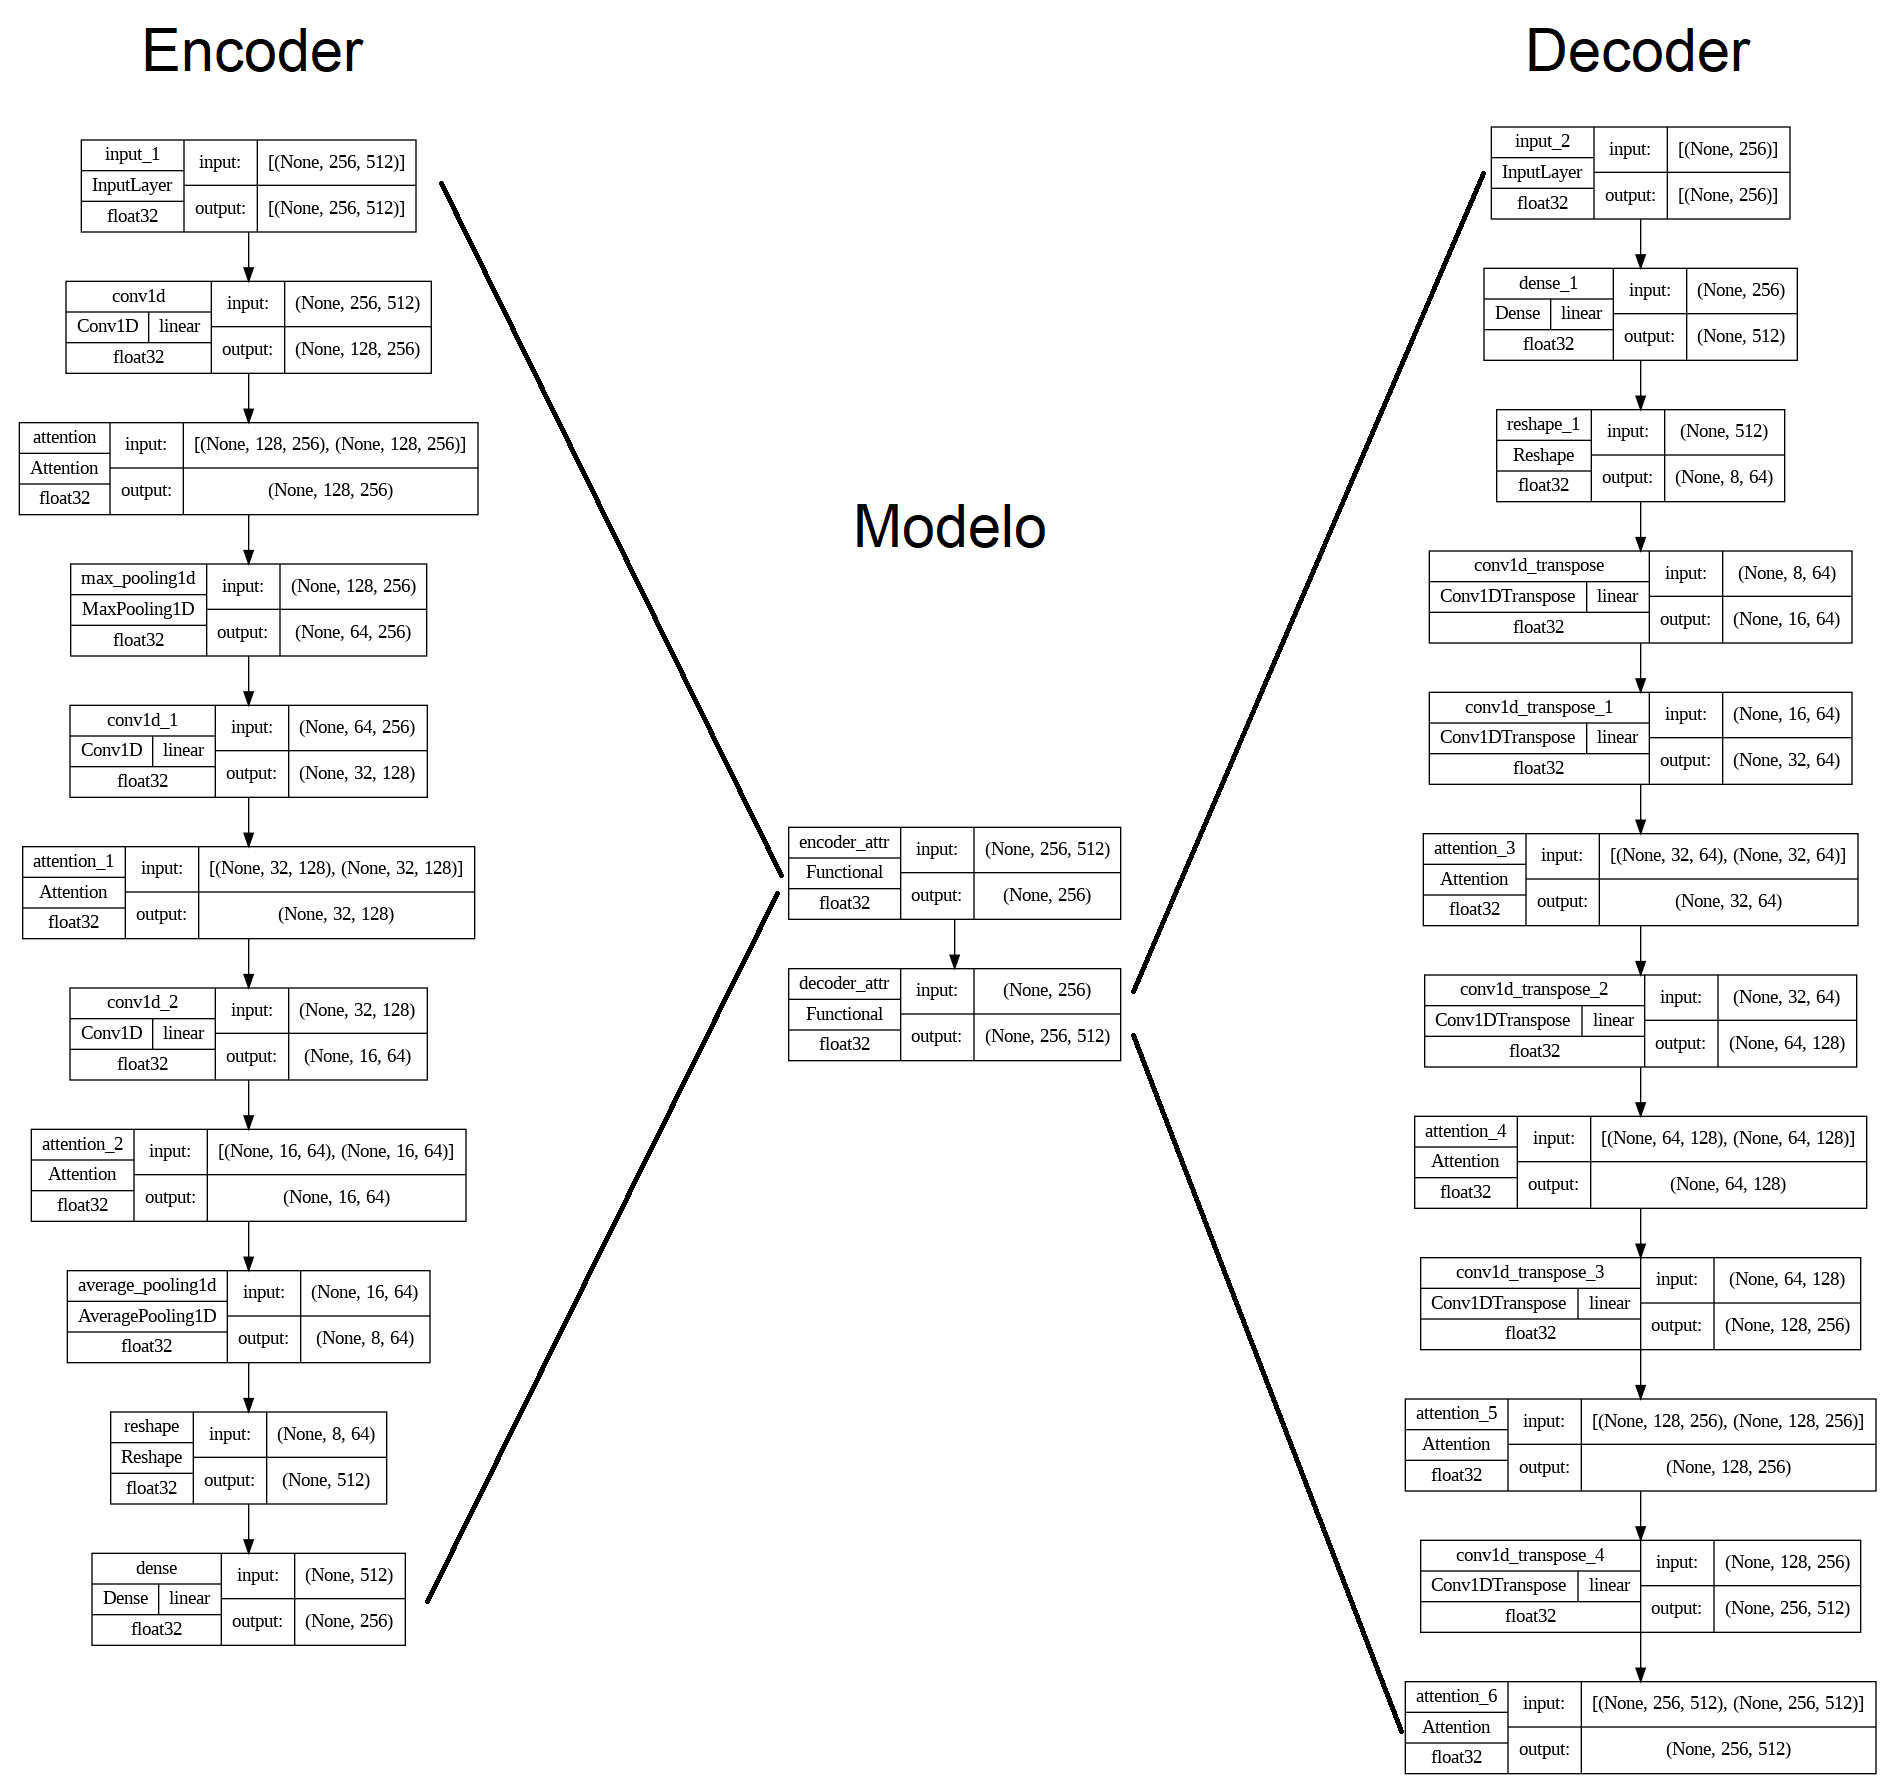
\includegraphics[width=\linewidth]{architecture.png}
	\caption{Arquitectura encoder-decoder para el vectorización de recetas.}
	\label{fig:encoder_decoder}
\end{figure*}


\end{document}
